% CS604 final report (Team 06), written with the ICLR 2026 template (iclr2026_conference.sty).
% Compile: pdflatex -> bibtex -> pdflatex -> pdflatex (Overleaf), or locally: tectonic -X compile main.tex
% Page limit (course): main text at most 10 pages; references and the appendix follow it.

\documentclass{article} % For LaTeX2e
\PassOptionsToPackage{dvipsnames}{xcolor}
\usepackage{iclr2026_conference,times}

% XeLaTeX (e.g. tectonic) ignores the Type 1 Times fonts of the times package, so use the TeX Gyre clones
% (same metrics as Times/Helvetica/Courier). pdfLaTeX, as on Overleaf, skips this and keeps the template's fonts.
\usepackage{iftex}
\ifXeTeX
  \usepackage{fontspec}
  \setmainfont{texgyretermes}[Extension=.otf, UprightFont=*-regular, BoldFont=*-bold, ItalicFont=*-italic, BoldItalicFont=*-bolditalic]
  \setsansfont{texgyreheros}[Extension=.otf, UprightFont=*-regular, BoldFont=*-bold, ItalicFont=*-italic, BoldItalicFont=*-bolditalic]
  \setmonofont{texgyrecursor}[Extension=.otf, UprightFont=*-regular, BoldFont=*-bold, ItalicFont=*-italic, BoldItalicFont=*-bolditalic]
\fi

% Optional math commands from https://github.com/goodfeli/dlbook_notation.
%%%%% NEW MATH DEFINITIONS %%%%%

\usepackage{amsmath,amsfonts,bm}

% Mark sections of captions for referring to divisions of figures
\newcommand{\figleft}{{\em (Left)}}
\newcommand{\figcenter}{{\em (Center)}}
\newcommand{\figright}{{\em (Right)}}
\newcommand{\figtop}{{\em (Top)}}
\newcommand{\figbottom}{{\em (Bottom)}}
\newcommand{\captiona}{{\em (a)}}
\newcommand{\captionb}{{\em (b)}}
\newcommand{\captionc}{{\em (c)}}
\newcommand{\captiond}{{\em (d)}}

% Highlight a newly defined term
\newcommand{\newterm}[1]{{\bf #1}}


% Figure reference, lower-case.
\def\figref#1{figure~\ref{#1}}
% Figure reference, capital. For start of sentence
\def\Figref#1{Figure~\ref{#1}}
\def\twofigref#1#2{figures \ref{#1} and \ref{#2}}
\def\quadfigref#1#2#3#4{figures \ref{#1}, \ref{#2}, \ref{#3} and \ref{#4}}
% Section reference, lower-case.
\def\secref#1{section~\ref{#1}}
% Section reference, capital.
\def\Secref#1{Section~\ref{#1}}
% Reference to two sections.
\def\twosecrefs#1#2{sections \ref{#1} and \ref{#2}}
% Reference to three sections.
\def\secrefs#1#2#3{sections \ref{#1}, \ref{#2} and \ref{#3}}
% Reference to an equation, lower-case.
\def\eqref#1{equation~\ref{#1}}
% Reference to an equation, upper case
\def\Eqref#1{Equation~\ref{#1}}
% A raw reference to an equation---avoid using if possible
\def\plaineqref#1{\ref{#1}}
% Reference to a chapter, lower-case.
\def\chapref#1{chapter~\ref{#1}}
% Reference to an equation, upper case.
\def\Chapref#1{Chapter~\ref{#1}}
% Reference to a range of chapters
\def\rangechapref#1#2{chapters\ref{#1}--\ref{#2}}
% Reference to an algorithm, lower-case.
\def\algref#1{algorithm~\ref{#1}}
% Reference to an algorithm, upper case.
\def\Algref#1{Algorithm~\ref{#1}}
\def\twoalgref#1#2{algorithms \ref{#1} and \ref{#2}}
\def\Twoalgref#1#2{Algorithms \ref{#1} and \ref{#2}}
% Reference to a part, lower case
\def\partref#1{part~\ref{#1}}
% Reference to a part, upper case
\def\Partref#1{Part~\ref{#1}}
\def\twopartref#1#2{parts \ref{#1} and \ref{#2}}

\def\ceil#1{\lceil #1 \rceil}
\def\floor#1{\lfloor #1 \rfloor}
\def\1{\bm{1}}
\newcommand{\train}{\mathcal{D}}
\newcommand{\valid}{\mathcal{D_{\mathrm{valid}}}}
\newcommand{\test}{\mathcal{D_{\mathrm{test}}}}

\def\eps{{\epsilon}}


% Random variables
\def\reta{{\textnormal{$\eta$}}}
\def\ra{{\textnormal{a}}}
\def\rb{{\textnormal{b}}}
\def\rc{{\textnormal{c}}}
\def\rd{{\textnormal{d}}}
\def\re{{\textnormal{e}}}
\def\rf{{\textnormal{f}}}
\def\rg{{\textnormal{g}}}
\def\rh{{\textnormal{h}}}
\def\ri{{\textnormal{i}}}
\def\rj{{\textnormal{j}}}
\def\rk{{\textnormal{k}}}
\def\rl{{\textnormal{l}}}
% rm is already a command, just don't name any random variables m
\def\rn{{\textnormal{n}}}
\def\ro{{\textnormal{o}}}
\def\rp{{\textnormal{p}}}
\def\rq{{\textnormal{q}}}
\def\rr{{\textnormal{r}}}
\def\rs{{\textnormal{s}}}
\def\rt{{\textnormal{t}}}
\def\ru{{\textnormal{u}}}
\def\rv{{\textnormal{v}}}
\def\rw{{\textnormal{w}}}
\def\rx{{\textnormal{x}}}
\def\ry{{\textnormal{y}}}
\def\rz{{\textnormal{z}}}

% Random vectors
\def\rvepsilon{{\mathbf{\epsilon}}}
\def\rvtheta{{\mathbf{\theta}}}
\def\rva{{\mathbf{a}}}
\def\rvb{{\mathbf{b}}}
\def\rvc{{\mathbf{c}}}
\def\rvd{{\mathbf{d}}}
\def\rve{{\mathbf{e}}}
\def\rvf{{\mathbf{f}}}
\def\rvg{{\mathbf{g}}}
\def\rvh{{\mathbf{h}}}
\def\rvu{{\mathbf{i}}}
\def\rvj{{\mathbf{j}}}
\def\rvk{{\mathbf{k}}}
\def\rvl{{\mathbf{l}}}
\def\rvm{{\mathbf{m}}}
\def\rvn{{\mathbf{n}}}
\def\rvo{{\mathbf{o}}}
\def\rvp{{\mathbf{p}}}
\def\rvq{{\mathbf{q}}}
\def\rvr{{\mathbf{r}}}
\def\rvs{{\mathbf{s}}}
\def\rvt{{\mathbf{t}}}
\def\rvu{{\mathbf{u}}}
\def\rvv{{\mathbf{v}}}
\def\rvw{{\mathbf{w}}}
\def\rvx{{\mathbf{x}}}
\def\rvy{{\mathbf{y}}}
\def\rvz{{\mathbf{z}}}

% Elements of random vectors
\def\erva{{\textnormal{a}}}
\def\ervb{{\textnormal{b}}}
\def\ervc{{\textnormal{c}}}
\def\ervd{{\textnormal{d}}}
\def\erve{{\textnormal{e}}}
\def\ervf{{\textnormal{f}}}
\def\ervg{{\textnormal{g}}}
\def\ervh{{\textnormal{h}}}
\def\ervi{{\textnormal{i}}}
\def\ervj{{\textnormal{j}}}
\def\ervk{{\textnormal{k}}}
\def\ervl{{\textnormal{l}}}
\def\ervm{{\textnormal{m}}}
\def\ervn{{\textnormal{n}}}
\def\ervo{{\textnormal{o}}}
\def\ervp{{\textnormal{p}}}
\def\ervq{{\textnormal{q}}}
\def\ervr{{\textnormal{r}}}
\def\ervs{{\textnormal{s}}}
\def\ervt{{\textnormal{t}}}
\def\ervu{{\textnormal{u}}}
\def\ervv{{\textnormal{v}}}
\def\ervw{{\textnormal{w}}}
\def\ervx{{\textnormal{x}}}
\def\ervy{{\textnormal{y}}}
\def\ervz{{\textnormal{z}}}

% Random matrices
\def\rmA{{\mathbf{A}}}
\def\rmB{{\mathbf{B}}}
\def\rmC{{\mathbf{C}}}
\def\rmD{{\mathbf{D}}}
\def\rmE{{\mathbf{E}}}
\def\rmF{{\mathbf{F}}}
\def\rmG{{\mathbf{G}}}
\def\rmH{{\mathbf{H}}}
\def\rmI{{\mathbf{I}}}
\def\rmJ{{\mathbf{J}}}
\def\rmK{{\mathbf{K}}}
\def\rmL{{\mathbf{L}}}
\def\rmM{{\mathbf{M}}}
\def\rmN{{\mathbf{N}}}
\def\rmO{{\mathbf{O}}}
\def\rmP{{\mathbf{P}}}
\def\rmQ{{\mathbf{Q}}}
\def\rmR{{\mathbf{R}}}
\def\rmS{{\mathbf{S}}}
\def\rmT{{\mathbf{T}}}
\def\rmU{{\mathbf{U}}}
\def\rmV{{\mathbf{V}}}
\def\rmW{{\mathbf{W}}}
\def\rmX{{\mathbf{X}}}
\def\rmY{{\mathbf{Y}}}
\def\rmZ{{\mathbf{Z}}}

% Elements of random matrices
\def\ermA{{\textnormal{A}}}
\def\ermB{{\textnormal{B}}}
\def\ermC{{\textnormal{C}}}
\def\ermD{{\textnormal{D}}}
\def\ermE{{\textnormal{E}}}
\def\ermF{{\textnormal{F}}}
\def\ermG{{\textnormal{G}}}
\def\ermH{{\textnormal{H}}}
\def\ermI{{\textnormal{I}}}
\def\ermJ{{\textnormal{J}}}
\def\ermK{{\textnormal{K}}}
\def\ermL{{\textnormal{L}}}
\def\ermM{{\textnormal{M}}}
\def\ermN{{\textnormal{N}}}
\def\ermO{{\textnormal{O}}}
\def\ermP{{\textnormal{P}}}
\def\ermQ{{\textnormal{Q}}}
\def\ermR{{\textnormal{R}}}
\def\ermS{{\textnormal{S}}}
\def\ermT{{\textnormal{T}}}
\def\ermU{{\textnormal{U}}}
\def\ermV{{\textnormal{V}}}
\def\ermW{{\textnormal{W}}}
\def\ermX{{\textnormal{X}}}
\def\ermY{{\textnormal{Y}}}
\def\ermZ{{\textnormal{Z}}}

% Vectors
\def\vzero{{\bm{0}}}
\def\vone{{\bm{1}}}
\def\vmu{{\bm{\mu}}}
\def\vtheta{{\bm{\theta}}}
\def\va{{\bm{a}}}
\def\vb{{\bm{b}}}
\def\vc{{\bm{c}}}
\def\vd{{\bm{d}}}
\def\ve{{\bm{e}}}
\def\vf{{\bm{f}}}
\def\vg{{\bm{g}}}
\def\vh{{\bm{h}}}
\def\vi{{\bm{i}}}
\def\vj{{\bm{j}}}
\def\vk{{\bm{k}}}
\def\vl{{\bm{l}}}
\def\vm{{\bm{m}}}
\def\vn{{\bm{n}}}
\def\vo{{\bm{o}}}
\def\vp{{\bm{p}}}
\def\vq{{\bm{q}}}
\def\vr{{\bm{r}}}
\def\vs{{\bm{s}}}
\def\vt{{\bm{t}}}
\def\vu{{\bm{u}}}
\def\vv{{\bm{v}}}
\def\vw{{\bm{w}}}
\def\vx{{\bm{x}}}
\def\vy{{\bm{y}}}
\def\vz{{\bm{z}}}

% Elements of vectors
\def\evalpha{{\alpha}}
\def\evbeta{{\beta}}
\def\evepsilon{{\epsilon}}
\def\evlambda{{\lambda}}
\def\evomega{{\omega}}
\def\evmu{{\mu}}
\def\evpsi{{\psi}}
\def\evsigma{{\sigma}}
\def\evtheta{{\theta}}
\def\eva{{a}}
\def\evb{{b}}
\def\evc{{c}}
\def\evd{{d}}
\def\eve{{e}}
\def\evf{{f}}
\def\evg{{g}}
\def\evh{{h}}
\def\evi{{i}}
\def\evj{{j}}
\def\evk{{k}}
\def\evl{{l}}
\def\evm{{m}}
\def\evn{{n}}
\def\evo{{o}}
\def\evp{{p}}
\def\evq{{q}}
\def\evr{{r}}
\def\evs{{s}}
\def\evt{{t}}
\def\evu{{u}}
\def\evv{{v}}
\def\evw{{w}}
\def\evx{{x}}
\def\evy{{y}}
\def\evz{{z}}

% Matrix
\def\mA{{\bm{A}}}
\def\mB{{\bm{B}}}
\def\mC{{\bm{C}}}
\def\mD{{\bm{D}}}
\def\mE{{\bm{E}}}
\def\mF{{\bm{F}}}
\def\mG{{\bm{G}}}
\def\mH{{\bm{H}}}
\def\mI{{\bm{I}}}
\def\mJ{{\bm{J}}}
\def\mK{{\bm{K}}}
\def\mL{{\bm{L}}}
\def\mM{{\bm{M}}}
\def\mN{{\bm{N}}}
\def\mO{{\bm{O}}}
\def\mP{{\bm{P}}}
\def\mQ{{\bm{Q}}}
\def\mR{{\bm{R}}}
\def\mS{{\bm{S}}}
\def\mT{{\bm{T}}}
\def\mU{{\bm{U}}}
\def\mV{{\bm{V}}}
\def\mW{{\bm{W}}}
\def\mX{{\bm{X}}}
\def\mY{{\bm{Y}}}
\def\mZ{{\bm{Z}}}
\def\mBeta{{\bm{\beta}}}
\def\mPhi{{\bm{\Phi}}}
\def\mLambda{{\bm{\Lambda}}}
\def\mSigma{{\bm{\Sigma}}}

% Tensor
\DeclareMathAlphabet{\mathsfit}{\encodingdefault}{\sfdefault}{m}{sl}
\SetMathAlphabet{\mathsfit}{bold}{\encodingdefault}{\sfdefault}{bx}{n}
\newcommand{\tens}[1]{\bm{\mathsfit{#1}}}
\def\tA{{\tens{A}}}
\def\tB{{\tens{B}}}
\def\tC{{\tens{C}}}
\def\tD{{\tens{D}}}
\def\tE{{\tens{E}}}
\def\tF{{\tens{F}}}
\def\tG{{\tens{G}}}
\def\tH{{\tens{H}}}
\def\tI{{\tens{I}}}
\def\tJ{{\tens{J}}}
\def\tK{{\tens{K}}}
\def\tL{{\tens{L}}}
\def\tM{{\tens{M}}}
\def\tN{{\tens{N}}}
\def\tO{{\tens{O}}}
\def\tP{{\tens{P}}}
\def\tQ{{\tens{Q}}}
\def\tR{{\tens{R}}}
\def\tS{{\tens{S}}}
\def\tT{{\tens{T}}}
\def\tU{{\tens{U}}}
\def\tV{{\tens{V}}}
\def\tW{{\tens{W}}}
\def\tX{{\tens{X}}}
\def\tY{{\tens{Y}}}
\def\tZ{{\tens{Z}}}


% Graph
\def\gA{{\mathcal{A}}}
\def\gB{{\mathcal{B}}}
\def\gC{{\mathcal{C}}}
\def\gD{{\mathcal{D}}}
\def\gE{{\mathcal{E}}}
\def\gF{{\mathcal{F}}}
\def\gG{{\mathcal{G}}}
\def\gH{{\mathcal{H}}}
\def\gI{{\mathcal{I}}}
\def\gJ{{\mathcal{J}}}
\def\gK{{\mathcal{K}}}
\def\gL{{\mathcal{L}}}
\def\gM{{\mathcal{M}}}
\def\gN{{\mathcal{N}}}
\def\gO{{\mathcal{O}}}
\def\gP{{\mathcal{P}}}
\def\gQ{{\mathcal{Q}}}
\def\gR{{\mathcal{R}}}
\def\gS{{\mathcal{S}}}
\def\gT{{\mathcal{T}}}
\def\gU{{\mathcal{U}}}
\def\gV{{\mathcal{V}}}
\def\gW{{\mathcal{W}}}
\def\gX{{\mathcal{X}}}
\def\gY{{\mathcal{Y}}}
\def\gZ{{\mathcal{Z}}}

% Sets
\def\sA{{\mathbb{A}}}
\def\sB{{\mathbb{B}}}
\def\sC{{\mathbb{C}}}
\def\sD{{\mathbb{D}}}
% Don't use a set called E, because this would be the same as our symbol
% for expectation.
\def\sF{{\mathbb{F}}}
\def\sG{{\mathbb{G}}}
\def\sH{{\mathbb{H}}}
\def\sI{{\mathbb{I}}}
\def\sJ{{\mathbb{J}}}
\def\sK{{\mathbb{K}}}
\def\sL{{\mathbb{L}}}
\def\sM{{\mathbb{M}}}
\def\sN{{\mathbb{N}}}
\def\sO{{\mathbb{O}}}
\def\sP{{\mathbb{P}}}
\def\sQ{{\mathbb{Q}}}
\def\sR{{\mathbb{R}}}
\def\sS{{\mathbb{S}}}
\def\sT{{\mathbb{T}}}
\def\sU{{\mathbb{U}}}
\def\sV{{\mathbb{V}}}
\def\sW{{\mathbb{W}}}
\def\sX{{\mathbb{X}}}
\def\sY{{\mathbb{Y}}}
\def\sZ{{\mathbb{Z}}}

% Entries of a matrix
\def\emLambda{{\Lambda}}
\def\emA{{A}}
\def\emB{{B}}
\def\emC{{C}}
\def\emD{{D}}
\def\emE{{E}}
\def\emF{{F}}
\def\emG{{G}}
\def\emH{{H}}
\def\emI{{I}}
\def\emJ{{J}}
\def\emK{{K}}
\def\emL{{L}}
\def\emM{{M}}
\def\emN{{N}}
\def\emO{{O}}
\def\emP{{P}}
\def\emQ{{Q}}
\def\emR{{R}}
\def\emS{{S}}
\def\emT{{T}}
\def\emU{{U}}
\def\emV{{V}}
\def\emW{{W}}
\def\emX{{X}}
\def\emY{{Y}}
\def\emZ{{Z}}
\def\emSigma{{\Sigma}}

% entries of a tensor
% Same font as tensor, without \bm wrapper
\newcommand{\etens}[1]{\mathsfit{#1}}
\def\etLambda{{\etens{\Lambda}}}
\def\etA{{\etens{A}}}
\def\etB{{\etens{B}}}
\def\etC{{\etens{C}}}
\def\etD{{\etens{D}}}
\def\etE{{\etens{E}}}
\def\etF{{\etens{F}}}
\def\etG{{\etens{G}}}
\def\etH{{\etens{H}}}
\def\etI{{\etens{I}}}
\def\etJ{{\etens{J}}}
\def\etK{{\etens{K}}}
\def\etL{{\etens{L}}}
\def\etM{{\etens{M}}}
\def\etN{{\etens{N}}}
\def\etO{{\etens{O}}}
\def\etP{{\etens{P}}}
\def\etQ{{\etens{Q}}}
\def\etR{{\etens{R}}}
\def\etS{{\etens{S}}}
\def\etT{{\etens{T}}}
\def\etU{{\etens{U}}}
\def\etV{{\etens{V}}}
\def\etW{{\etens{W}}}
\def\etX{{\etens{X}}}
\def\etY{{\etens{Y}}}
\def\etZ{{\etens{Z}}}

% The true underlying data generating distribution
\newcommand{\pdata}{p_{\rm{data}}}
% The empirical distribution defined by the training set
\newcommand{\ptrain}{\hat{p}_{\rm{data}}}
\newcommand{\Ptrain}{\hat{P}_{\rm{data}}}
% The model distribution
\newcommand{\pmodel}{p_{\rm{model}}}
\newcommand{\Pmodel}{P_{\rm{model}}}
\newcommand{\ptildemodel}{\tilde{p}_{\rm{model}}}
% Stochastic autoencoder distributions
\newcommand{\pencode}{p_{\rm{encoder}}}
\newcommand{\pdecode}{p_{\rm{decoder}}}
\newcommand{\precons}{p_{\rm{reconstruct}}}

\newcommand{\laplace}{\mathrm{Laplace}} % Laplace distribution

\newcommand{\E}{\mathbb{E}}
\newcommand{\Ls}{\mathcal{L}}
\newcommand{\R}{\mathbb{R}}
\newcommand{\emp}{\tilde{p}}
\newcommand{\lr}{\alpha}
\newcommand{\reg}{\lambda}
\newcommand{\rect}{\mathrm{rectifier}}
\newcommand{\softmax}{\mathrm{softmax}}
\newcommand{\sigmoid}{\sigma}
\newcommand{\softplus}{\zeta}
\newcommand{\KL}{D_{\mathrm{KL}}}
\newcommand{\Var}{\mathrm{Var}}
\newcommand{\standarderror}{\mathrm{SE}}
\newcommand{\Cov}{\mathrm{Cov}}
% Wolfram Mathworld says $L^2$ is for function spaces and $\ell^2$ is for vectors
% But then they seem to use $L^2$ for vectors throughout the site, and so does
% wikipedia.
\newcommand{\normlzero}{L^0}
\newcommand{\normlone}{L^1}
\newcommand{\normltwo}{L^2}
\newcommand{\normlp}{L^p}
\newcommand{\normmax}{L^\infty}

\newcommand{\parents}{Pa} % See usage in notation.tex. Chosen to match Daphne's book.

\DeclareMathOperator*{\argmax}{arg\,max}
\DeclareMathOperator*{\argmin}{arg\,min}

\DeclareMathOperator{\sign}{sign}
\DeclareMathOperator{\Tr}{Tr}
\let\ab\allowbreak


\usepackage{hyperref}
\usepackage{url}
\usepackage{amsmath,amssymb}
\usepackage{booktabs,multirow,tabularx}
\usepackage{float}  % [H] keeps the appendix tables under their headings
\usepackage{graphicx}
\usepackage{xcolor}
\usepackage[shortlabels,inline]{enumitem}
\usepackage{microtype}
\usepackage[capitalize]{cleveref}
\definecolor{linkblue}{rgb}{0.16,0.40,0.69}
\hypersetup{colorlinks=true,allcolors=linkblue}
\usepackage{xspace}

% Short forms used in the text
\makeatletter
\DeclareRobustCommand\onedot{\futurelet\@let@token\@onedot}
\def\@onedot{\ifx\@let@token.\else.\null\fi\xspace}
\makeatother
\def\ie{\emph{i.e}\onedot} \def\eg{\emph{e.g}\onedot} \def\vs{\emph{vs}\onedot}
\newcommand{\todo}[1]{{\color{red}#1}}          % placeholders still to fill in
% \renewcommand{\todo}[1]{#1}                  % uncomment when all placeholders are filled
\newcommand{\run}[1]{\texttt{#1}}               % run identifiers (escape underscores as \_)
\newcommand{\minus}{\ensuremath{-}}

\title{Prototype-Initialized Adaptation of ViT-B/16 for 10,000-Class Fine-Grained Classification under a Fixed Compute Budget}

\author{\todo{Member 1}, \todo{Member 2}, \todo{Member 3} \& \todo{Member 4} \\
CS604 Team 06, Singapore Management University \\
\texttt{\todo{\{email addresses\}}}
}

\iclrfinalcopy % show the author names (course report, not an anonymous submission)

\begin{document}

\maketitle
% The template's final-copy header says "Published as a conference paper at ICLR 2026"; this is a course report.
\lhead{CS604 Project Report, Team 06}

\begin{abstract}
We adapt ViT-B/16 to a fine-grained dataset with 10,000 classes and only 45 training images per class, with 2 hours on 48\,GB of GPU memory per training run.
We compare seven adaptation methods under the same settings, from a linear probe to full fine-tuning, BitFit, Adapter, AdaptFormer and LoRA.
The choice that mattered most was how to start the new 10,000-class head.
The usual start, a linear probe trained on frozen features of the training images, made all three methods we tested worse; starting each class from its mean feature (a prototype) gave 2.1--3.1 points more.
We also find that where the trainable parameters are matters more than how many there are: LoRA on 1.375\% of the backbone matches fine-tuning the last four blocks (33\%).
Our final full fine-tuning model reaches 76.22\% top-1 on the CodaBench validation set and 76.09\% on the test set (reference: 70.8\%) in 1.03 GPU-hours, and our final LoRA model reaches 71.90\% and 71.67\% (reference LoRA: 68.3\%) with no extra inference cost.
We also report the ideas that failed, and show after the deadline that larger input images add another 4.4 points.
\end{abstract}

\section{Introduction}
\label{sec:intro}

Pretrained Vision Transformers \citep{dosovitskiy2021vit,steiner2022augreg} are usually adapted to a new task instead of being trained from scratch, either by fine-tuning all weights or by training a small number of added parameters \citep{houlsby2019adapter,hu2022lora,chen2022adaptformer}.
In this project we adapt ViT-B/16 to a fine-grained dataset with 10,000 classes whose names are hidden.
There are 45 training images per class (450,000 in total); the labels of the validation set (50,000 images) and the test set (100,000 images) are hidden and scored on CodaBench.
Each training run may use 2 hours on 48\,GB of GPU memory, which is 1.2 hours on our 80\,GB A100.

\begin{figure}[b]
  \centering
  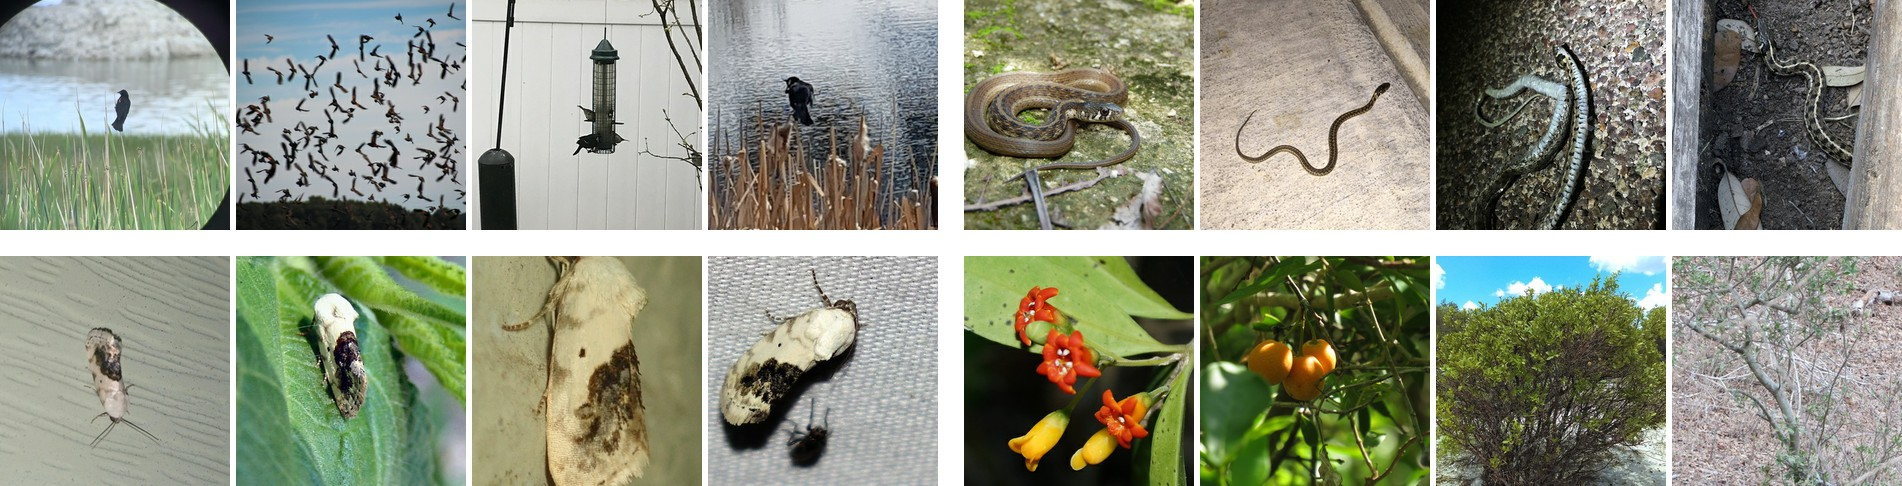
\includegraphics[width=\linewidth]{figures/data_examples_wide.jpg}
  \caption{\textbf{Training images of four of the 10,000 classes.} Each group of four is one class (a bird, a snake, a moth and a plant): one bird or a whole flock, a flower or a whole shrub. Each class has only 45 such images.}
  \label{fig:examples}
\end{figure}

\paragraph{Why this is hard.}
As \cref{fig:examples} shows, one class can look very different from image to image, while different classes in a fine-grained dataset can look alike, and each class has only 45 images.
A model can easily memorize such a small set, so a low training loss tells us little; every choice has to be judged on held-out images.
The new classifier head is also large: a $10{,}000 \times 768$ layer has 7.69M parameters, 9\% of the 85.8M-parameter backbone, and each of its rows is trained on only 43--45 images.
Finally, the budget is tight: one epoch of full fine-tuning takes about 7 minutes, so only about eight epochs fit into one run.

\paragraph{Our objectives.}
A high leaderboard score was not our only goal.
We wanted to answer three questions.
(1)~What limits accuracy when there are many classes but few images per class, and how can we fix it?
(2)~If we compare adaptation methods fairly, with one protocol and one budget, where do trainable parameters help most, and what does each method cost in memory and latency?
(3)~How should a fixed budget be split between epochs, training data and test-time computation?
We answered them with 26 runs, each changing one setting, and chose models on a local holdout split that matches the CodaBench validation score within 0.3 points.
Our contributions are:
\begin{itemize}[leftmargin=*,itemsep=1pt,topsep=2pt]
    \item \textbf{A better start for the head.} The linear-probe (LP) head used by LP-FT \citep{kumar2022lpft}, trained on frozen features of the training images, hurts in our task. Starting each class from its normalized mean feature (a prototype) instead adds 2.1--3.1 points for full fine-tuning, LoRA and AdaptFormer. A random-head control shows that the harm comes from fitting the head on the training images (\cref{sec:ablation-head}).
    \item \textbf{A fair comparison of seven adaptation methods.} Small changes in every block give much more accuracy per parameter than fine-tuning the top blocks: LoRA on 1.375\% of the backbone matches the last four blocks (33\%). Training memory depends on how far back the gradients go, not on how many parameters are trained (\cref{sec:compare}).
    \item \textbf{Final results with their full cost.} Our final models reach 76.22\% (full fine-tuning, $+$5.4 over the reference) and 71.90\% (LoRA, $+$3.6 over the reference LoRA) on the validation set, and 76.09\% and 71.67\% on the test set, within the budget (\cref{sec:main}).
    \item \textbf{The process, including failures.} We report the study round by round, with the ideas that failed (\cref{sec:process}), and find after the deadline that larger input images add 4.4 points (\cref{sec:post}).
\end{itemize}

\section{Related Work}
\label{sec:related}

\paragraph{Pretrained ViTs and fine-tuning.}
ViT \citep{dosovitskiy2021vit} applies a Transformer \citep{vaswani2017attention} to $16 \times 16$ image patches.
Pretraining on ImageNet-21k \citep{deng2009imagenet} with strong augmentation and regularization (AugReg, \citealp{steiner2022augreg}) gives backbones that transfer well, and models that are better on ImageNet also transfer better \citep{kornblith2019better}.
Common fine-tuning recipes use AdamW \citep{loshchilov2019adamw}, warmup with cosine decay \citep{loshchilov2017sgdr}, label smoothing \citep{szegedy2016rethinking}, stochastic depth \citep{huang2016stochastic} and layer-wise learning-rate decay \citep{bao2022beit}; our full fine-tuning recipe uses all of them.

\paragraph{Parameter-efficient fine-tuning (PEFT).}
PEFT methods train only a small part of the model.
The oldest option is to train only the top layers, whose features are the most task-specific \citep{yosinski2014transferable}.
BitFit \citep{benzaken2022bitfit} trains only the bias terms.
Adapters \citep{houlsby2019adapter} add a small bottleneck MLP to every block, and AdaptFormer \citep{chen2022adaptformer} puts a scaled bottleneck next to the MLP instead of after it.
LoRA \citep{hu2022lora} learns a low-rank update $\Delta W = BA$ of frozen weight matrices, which can be merged into the weights after training.
VPT \citep{jia2022vpt} and prefix tuning \citep{li2021prefix} add learnable tokens instead.
\Cref{tab:related} lists the pros and cons we expected from the literature.
No method is best on every count: they trade accuracy against training memory, stored size and inference latency, so we measure all of these.

\paragraph{Starting the classifier head.}
When a pretrained model is moved to new classes, its head is replaced; ViT starts the new head at zero \citep{dosovitskiy2021vit}.
LP-FT \citep{kumar2022lpft} argues that a random head distorts the pretrained features during fine-tuning, which hurts accuracy on new domains.
It therefore first trains a linear probe on frozen features and then fine-tunes everything.
Prototypical networks \citep{snell2017prototypical} represent each class by the mean feature of its examples, and weight imprinting \citep{qi2018imprinted} copies normalized class means directly into the weights of a cosine classifier, to add new classes from a few examples.
We use imprinting as the starting head for full fine-tuning and PEFT, and compare it with LP-FT in a setting with many classes (10,000), few images per class (45) and a short budget.

\begin{table}[t]
  \caption{\textbf{Adaptation methods and head starts: pros and cons}, as expected from the literature. Our measured numbers are in \cref{sec:experiments}.}
  \label{tab:related}
  \centering
  \footnotesize
  \setlength{\tabcolsep}{4pt}
  \begin{tabularx}{\linewidth}{@{}l>{\raggedright}X>{\raggedright\arraybackslash}X@{}}
    \toprule
    Approach & Pros & Cons \\
    \midrule
    Full fine-tuning & most accurate with enough data & most memory; a full model copy per task \\
    Linear probe & cheapest; no backbone gradients & the features never adapt \\
    Top-$K$ blocks & little memory (short backward pass) & the lower blocks never adapt \\
    BitFit & tiny; no extra latency & little capacity \\
    Adapter & small; flexible & extra layers slow down inference \\
    AdaptFormer & small; keeps the MLP output & cannot be merged; slower inference \\
    LoRA & small; merged after training, no extra latency & gradients still pass through every block \\
    VPT, prefix tuning & very small & longer input, so slower; needs tuning of the token count \\
    \midrule
    Random or zero head & simple & large, noisy gradients at the start \\
    LP-FT head & protects the pretrained features & fitted on the training images (hurts here, \cref{sec:ablation-head}) \\
    Imprinted prototypes & no training; uses the class structure & only as good as the frozen features \\
    \bottomrule
  \end{tabularx}
\end{table}

\section{Method}
\label{sec:method}

\begin{figure}[t]
  \centering
  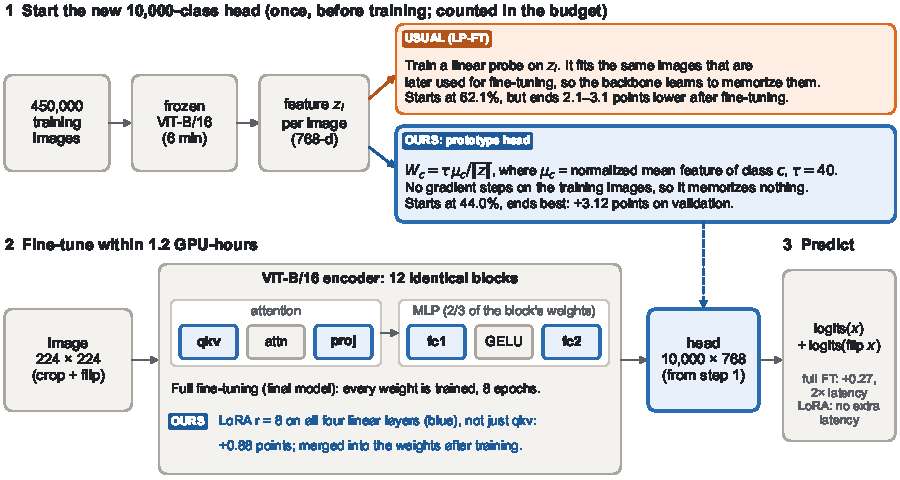
\includegraphics[width=\linewidth]{figures/fig_pipeline.pdf}
  \caption{\textbf{Our pipeline, with our changes in blue.}
  (1)~We start the new head from class prototypes of the frozen backbone, not from the usual LP-FT linear probe (orange), which is fitted on the same training images.
  (2)~We fine-tune all weights, or LoRA on all four linear layers (the reference: qkv only).
  (3)~Full fine-tuning adds the logits of each image and its mirror image. Gains are from \cref{sec:experiments}.}
  \label{fig:pipeline}
\end{figure}

\Cref{fig:pipeline} shows our pipeline.
Let $f_\theta$ map an image $x$ to its final \texttt{[CLS]} feature $z = f_\theta(x) \in \mathbb{R}^{768}$, and let $h(z) = Wz + b$ with $W \in \mathbb{R}^{10000 \times 768}$ be the new head.

\paragraph{What we changed, and why.}
We started from the recipes in the project description and changed five things, each after a test on the holdout (\cref{sec:process}):
\begin{enumerate}[leftmargin=*,itemsep=1pt,topsep=2pt]
  \item \textbf{A prototype head instead of a linear-probe head} (\cref{sec:head-init}). Our first runs used LP-FT. When LoRA's training loss went \emph{up} in its first epoch, we traced the problem to the probe, which had been fitted on the same images. A prototype head is not trained on them at all. This is our main change: $+$2.1 to $+$3.1 points.
  \item \textbf{LoRA on all four linear layers, not only qkv}, because the MLP holds two thirds of each block's weights: $+$0.88 points with 1.375\% of the backbone.
  \item \textbf{A different schedule for each final model}: 8 epochs for full fine-tuning, which keeps improving, and 3 for LoRA, which gets worse with more epochs (\cref{sec:ablation-lora}).
  \item \textbf{A budget clock that counts every GPU second}, including the feature extraction for the head, and shortens the schedule if a run would go over the budget (\cref{sec:budget}).
  \item \textbf{Flip test-time augmentation} for the full fine-tuning model: $+$0.27 points for twice the latency.
\end{enumerate}

\subsection{Backbone and budget}
\label{sec:budget}

\paragraph{Backbone.}
We use the timm \citep{wightman2019timm} checkpoint \nolinkurl{vit_base_patch16_224.augreg2_in21k_ft_in1k}, the backbone that the project description recommends: ViT-B/16 pretrained on ImageNet-21k with AugReg and fine-tuned on ImageNet-1k.
It has 85,798,656 parameters; its 1,000-class head is replaced by a new 10,000-class head (7,690,000 parameters).
We keep it in every experiment: after the deadline we checked two ImageNet-21k-only ViT-B/16 models that the project description also lists, and a linear probe on their frozen features is worse on our holdout (61.05\% and 51.07\% \vs 61.94\%).

\paragraph{Compute budget.}
The project allows 2\,h$\times$48\,GB $=$ 96\,GB$\cdot$h per training run ($\pm$10\%), which is 1.2 hours on our 80\,GB A100.
Our clock counts all GPU work for training (head initialization with feature extraction, all optimizer steps and the holdout check after every epoch), but not unpacking the data, saving checkpoints or the final predictions.
The code times training steps 20--120; if the planned epochs would use more than 97\% of the budget, it shortens the cosine schedule, and it stops training at 1.05$\times$ the budget.
Every run in our results finished within 1.06 GPU-hours; the only longer run is a post-deadline test that is not part of our results (\cref{sec:post}).

\subsection{Starting the 10,000-class head}
\label{sec:head-init}

The head is the largest new part of the model, and each of its rows is trained on at most 45 images.
A random head gives almost uniform logits (initial loss $\approx \ln 10000 = 9.2$), so early in training the backbone gets large, noisy gradients from it.
We compare three ways to start the head.

\paragraph{Random.} timm's default initialization of a new linear layer.

\paragraph{Prototype head (ours).}
With the frozen pretrained backbone, we extract the features $z_i$ of all training images once.
We then copy the L2-normalized class means into the head \citep{snell2017prototypical,qi2018imprinted}:
\begin{equation}
  \mu_c = \frac{\sum_{i:\,y_i=c} \hat z_i}{\big\|\sum_{i:\,y_i=c} \hat z_i\big\|}, \quad
  W_c = \frac{\tau}{\overline{\|z\|}}\, \mu_c, \quad b_c = 0,
  \label{eq:proto}
\end{equation}
where $\hat z_i = z_i / \|z_i\|$ and $\overline{\|z\|}$ is the mean feature norm, so each logit is about $\tau \cos(z, \mu_c)$.
We pick the temperature $\tau$ from $\{5, 10, 15, 20, 30, 40, 60, 80\}$ by the cross-entropy on 10,000 training features, which gives $\tau = 40$.
Without any training, this head already reaches 44.0\% holdout accuracy.
Feature extraction takes 6--7 minutes on an A100, and we count this time in every run's GPU-hours.
The head knows the class structure from the start, but it has never been fitted to single training images, so it has nothing to memorize.

\paragraph{Linear-probe (LP) head.}
Starting from the prototype head, we train $(W, b)$ on the cached frozen features for 10 epochs (AdamW, learning rate $10^{-3}$, weight decay $10^{-4}$, batch size 4,096, cosine decay, label smoothing 0.1).
This reaches 62.1\% holdout accuracy in a few seconds and is the first stage of LP-FT \citep{kumar2022lpft}.
It was our first design, chosen so that a random head would not distort the features.

\subsection{Adaptation methods}
\label{sec:peft}

\paragraph{Full fine-tuning.}
All backbone and head weights are trained with AdamW \citep{loshchilov2019adamw} at learning rate $10^{-4}$ and weight decay 0.05 (none on biases, normalization parameters, the class token and position embeddings).
We use layer-wise learning-rate decay of 0.75 \citep{bao2022beit}, drop path 0.1 \citep{huang2016stochastic}, a linear warmup (one epoch for runs of 6 or more epochs, 0.3 epochs for 3-epoch runs) and a cosine decay to zero \citep{loshchilov2017sgdr}.
Other settings are batch size 256, bf16 mixed precision, gradient clipping at norm 1 and label smoothing 0.1 \citep{szegedy2016rethinking}.
Training images get RandomResizedCrop (scale 0.25--1) and a horizontal flip; for evaluation, images are resized to 248 pixels and center-cropped to 224.
At test time, the final full fine-tuning model adds the logits of each image and of its horizontal flip \citep{krizhevsky2012imagenet}.

\paragraph{LoRA.}
For a frozen linear layer $W_0 \in \mathbb{R}^{d_\text{out} \times d_\text{in}}$, LoRA \citep{hu2022lora} computes
\begin{equation}
  y = W_0 x + \tfrac{\alpha}{r} B A x,
  \label{eq:lora}
\end{equation}
where $A \in \mathbb{R}^{r \times d_\text{in}}$ and $B \in \mathbb{R}^{d_\text{out} \times r}$ are trained and $B$ starts at zero, so training starts exactly from the pretrained model.
We use the PEFT library \citep{mangrulkar2022peft} with $r = 8$ and $\alpha = 16$.
timm joins the query, key and value projections into one \texttt{qkv} layer, so LoRA on \texttt{qkv} (294,912 parameters, 0.344\% of the backbone) adapts all three.
Our final LoRA model applies LoRA to all four linear layers of every block (\texttt{qkv}, \texttt{proj}, \texttt{fc1}, \texttt{fc2}), for 1,179,648 parameters (1.375\%).
The LoRA weights and the head use learning rate $10^{-3}$ and weight decay $10^{-4}$, with no LoRA dropout.
After training, $\tfrac{\alpha}{r}BA$ is added into $W_0$, so inference uses exactly the base model.

\paragraph{Other methods.}
AdaptFormer \citep{chen2022adaptformer} adds a bottleneck branch next to the MLP of each block,
\begin{equation}
  x_{l+1} = x' + \mathrm{MLP}(\mathrm{LN}(x')) + s \cdot W_\text{up}\,\mathrm{ReLU}(W_\text{down} x'),
  \label{eq:adaptformer}
\end{equation}
where $x'$ is the output of the attention sub-block; we use width 64, scale $s = 0.1$, dropout 0.1 and a zero-initialized $W_\text{up}$.
The serial Adapter \citep{houlsby2019adapter} applies the same bottleneck to the MLP output, before the residual addition and without a scale.
Both have 1,189,632 parameters (1.387\%) and cannot be merged into the backbone.
BitFit \citep{benzaken2022bitfit} trains only the bias vectors of all linear and normalization layers (102,912 parameters, 0.120\%).
Partial fine-tuning trains the last $K$ blocks and the final normalization layer; one block has 7,087,872 parameters (8.26\% of the backbone).
\Cref{tab:params} in the appendix shows how each count is computed.
In every run except zero-shot the head is also trained; since it alone has 7.69M parameters, we report trainable parameters without it, as in the project's 0.34\% LoRA reference.

\section{Experiments}
\label{sec:experiments}

\subsection{Setup}
\label{sec:setup}

\paragraph{Data and protocol.}
Validation and test labels are hidden, so we hold out 2 images per class from the training set (20,000 images, fixed seed).
We use this holdout to choose models and run ablations, and train on the other 43 images per class.
The final full fine-tuning model is then retrained on all 45 images per class; the final LoRA model keeps the holdout split and is trained on 43.
Validation and test images are used only to make submission files.
CodaBench reports top-1 accuracy; the validation set is balanced (5 images per class), so this is also the mean per-class accuracy.
Our holdout is close to the server score: 72.31\% \vs 72.57\% for full fine-tuning and 71.98\% \vs 71.90\% for LoRA.
At about 72\% accuracy on 20,000 images, the standard error is $\sqrt{0.72 \cdot 0.28 / 20{,}000} \approx 0.32$ points, so we treat differences below about 0.3 points as noise.
All runs use one seed.

\paragraph{Metrics.}
Latency is the mean time of one forward pass at batch size 1 on an A100 (bf16, 100 passes after 10 warm-up passes); for the same model it varies by up to about 0.5\,ms between runs.
Throughput is measured at batch size 256, GPU-hours come from the clock in \cref{sec:budget}, and memory is the peak allocated by PyTorch during training.
The appendix gives training-log excerpts, all runs, the hyperparameters and the hardware (\cref{sec:logs,sec:all-runs,sec:hparams,sec:hardware}).

\subsection{How we iterated}
\label{sec:process}

\begin{table}[t]
  \caption{\textbf{How we iterated}, one question per round (holdout top-1 unless marked val; FT: fine-tuning). $^*$After the deadline; no ranked submission uses it.}
  \label{tab:process}
  \centering
  \footnotesize
  \setlength{\tabcolsep}{4pt}
  \begin{tabularx}{\linewidth}{@{}l>{\raggedright}X>{\raggedright\arraybackslash}p{0.38\linewidth}@{}}
    \toprule
    Date & Question $\rightarrow$ experiment & Finding \\
    \midrule
    Sep 28 & Is our pipeline right? $\rightarrow$ reproduce the 3 references & all within 0.3 points \\
    Sep 28 & Do longer runs help? $\rightarrow$ full FT for 8 epochs, LoRA for 10 & full $+$1.4, LoRA $+$0.1; LoRA's loss goes up in epoch 1 \\
    Oct 18 & Is LoRA's learning rate too high? $\rightarrow$ halve it & \textbf{failed}: \minus0.12 (\cref{tab:peft}) \\
    Oct 18 & Does LoRA need more capacity? $\rightarrow$ adapt the MLP too & $+$0.88 (\cref{tab:peft}) \\
    Oct 19 & Is the LP head the problem? $\rightarrow$ LP \vs random \vs prototype & prototype $+$2.5; random ties it (\cref{tab:head}) \\
    Oct 19 & Final recipe $\rightarrow$ prototype head; full FT 8 ep.; LoRA 3 \vs 6 ep. & val 76.22, 71.90; LoRA 6 ep. \textbf{failed}: \minus0.46 \\
    Nov 2 & Which method is best per parameter? $\rightarrow$ seven methods, one protocol & small changes in every block (\cref{tab:compare}) \\
    Nov 5$^*$ & What limits us now? $\rightarrow$ in21k-only backbones; larger images & backbone: no gain; image size: $+$4.4 (\cref{tab:res}) \\
    \bottomrule
  \end{tabularx}
\end{table}

We ran the study in rounds; each round asked one question and changed one setting (\cref{tab:process}).
The failed ideas were useful too: when LoRA's training loss went up in its first epoch, we first blamed the learning rate, but halving it changed nothing, so we looked at the head next, which gave the largest gain of the project (\cref{sec:ablation-head}).

\paragraph{Reproducing the reference baselines.}
Before changing anything, we checked our pipeline against the three reference results in the project description.
Short 3-epoch runs with the LP head match all three within 0.3 points on our holdout (43.95\% \vs 43.7\% for the zero-shot prototype head, 70.88\% \vs 70.8\% for full fine-tuning, 68.57\% \vs 68.3\% for LoRA on qkv), so our pipeline and the way we count trainable parameters agree with the reference.

\subsection{Main results}
\label{sec:main}

\begin{table}[t]
  \caption{\textbf{Main results.}
  Holdout: 2 images per class held out from the training set; Val/Test: CodaBench validation/test (Phase 2).
  Params: trainable backbone parameters (share of the 85.8M backbone); the 10,000-class head (7.69M) is also trained in every row except zero-shot.
  Latency (ms, batch 1), throughput, GPU-hours and peak memory: one A100; LoRA after merging.
  $^\dagger$All 45 images per class; other rows (incl.\ the final LoRA model) use 43 and no TTA. $^\ddagger$Flip TTA (two forward passes; 7.35\,ms without).}
  \label{tab:main}
  \centering
  \scriptsize
  \setlength{\tabcolsep}{3pt}
  \begin{tabular}{@{}llcrrrrrrrr@{}}
    \toprule
    Method & Head & Ep. & Params & Holdout & Val & Test & ms & img/s & GPU-h & GB \\
    \midrule
    Zero-shot & prototype & 0 & 0 & 43.95 & -- & -- & 7.55 & 3,832 & 0.11 & 3.9 \\
    Linear probe & LP & -- & 0 & 62.07 & -- & -- & -- & -- & $\approx$0.11 & -- \\
    \midrule
    Full fine-tuning & LP & 8 & 85.8M (100\%) & 72.31 & 72.57 & -- & 7.35 & 3,864 & 1.03 & 18.9 \\
    \textbf{Full fine-tuning (final)}$^\dagger$ & prototype & 8 & 85.8M (100\%) & -- & \textbf{76.22} & \textbf{76.09} & 14.95$^\ddagger$ & 1,919$^\ddagger$ & 1.03 & 18.9 \\
    \midrule
    LoRA, qkv only & LP & 3 & 0.29M (0.344\%) & 68.57 & -- & -- & 7.22 & 3,817 & 0.40 & 13.5 \\
    AdaptFormer & LP & 3 & 1.19M (1.387\%) & 69.05 & -- & -- & 9.89 & 3,461 & 0.39 & 12.8 \\
    \textbf{LoRA, all linear (final)} & prototype & 3 & 1.18M (1.375\%) & \textbf{71.98} & \textbf{71.90} & \textbf{71.67} & 7.61 & 3,869 & 0.54 & 19.9 \\
    \bottomrule
  \end{tabular}
\end{table}

\Cref{tab:main} gives all four required metrics for the key models.
Our final full fine-tuning model reaches \textbf{76.22\%} on the CodaBench validation set, 5.4 points above the reference.
Changing one setting at a time (\cref{fig:progression,tab:length} in the appendix), replacing the LP head with the prototype head adds \textbf{3.12 points}, going from 3 to 8 epochs adds 2.21, flip TTA adds 0.27 (it changes 4.6\% of the predictions and doubles latency), and training on all 45 images per class adds 0.26 (close to the noise, but in the expected direction).
Our final LoRA model reaches \textbf{71.90\%} ($+$3.6 over the reference LoRA); it trains 1.375\% of the backbone, and after merging it has the same latency as the base model.
The two final models were not trained the same way: the LoRA model keeps the holdout split and uses no TTA.
Under the same settings (3 epochs, prototype head, holdout), LoRA reaches 98\% of the full fine-tuning accuracy (71.98\% \vs 73.38\%).
On the hidden test set (Phase 2), the two final models reach \textbf{76.09\%} and \textbf{71.67\%}, within 0.25 points of their validation scores.
Both models were fixed before the test set was released, and each used one of our two Phase 2 submissions.

\subsection{Starting the head}
\label{sec:ablation-head}

\begin{table}[t]
  \caption{\textbf{Head initialization} (top-1, \%); in each column only the head changes. Head alone: before training. Full FT 8 ep: all 45 images per class, flip TTA. $^*$RTX PRO 6000; the A100 rerun gives 71.98.}
  \label{tab:head}
  \centering
  \footnotesize
  \setlength{\tabcolsep}{5pt}
  \begin{tabular}{@{}lccccc@{}}
    \toprule
    & Head & LoRA, all linear & AdaptFormer & Full FT & Full FT \\
    Head init & alone & 3 ep, holdout & 3 ep, holdout & 3 ep, holdout & 8 ep, val \\
    \midrule
    Random & chance & 71.95$^*$ & -- & -- & -- \\
    Prototype (ours) & 44.0 & \textbf{72.00}$^*$ & \textbf{71.17} & \textbf{73.38} & \textbf{76.22} \\
    Linear probe (LP) & 62.1 & 69.45 & 69.05 & 70.88 & 73.10 \\
    \bottomrule
  \end{tabular}
\end{table}

\begin{figure}[t]
  \centering
  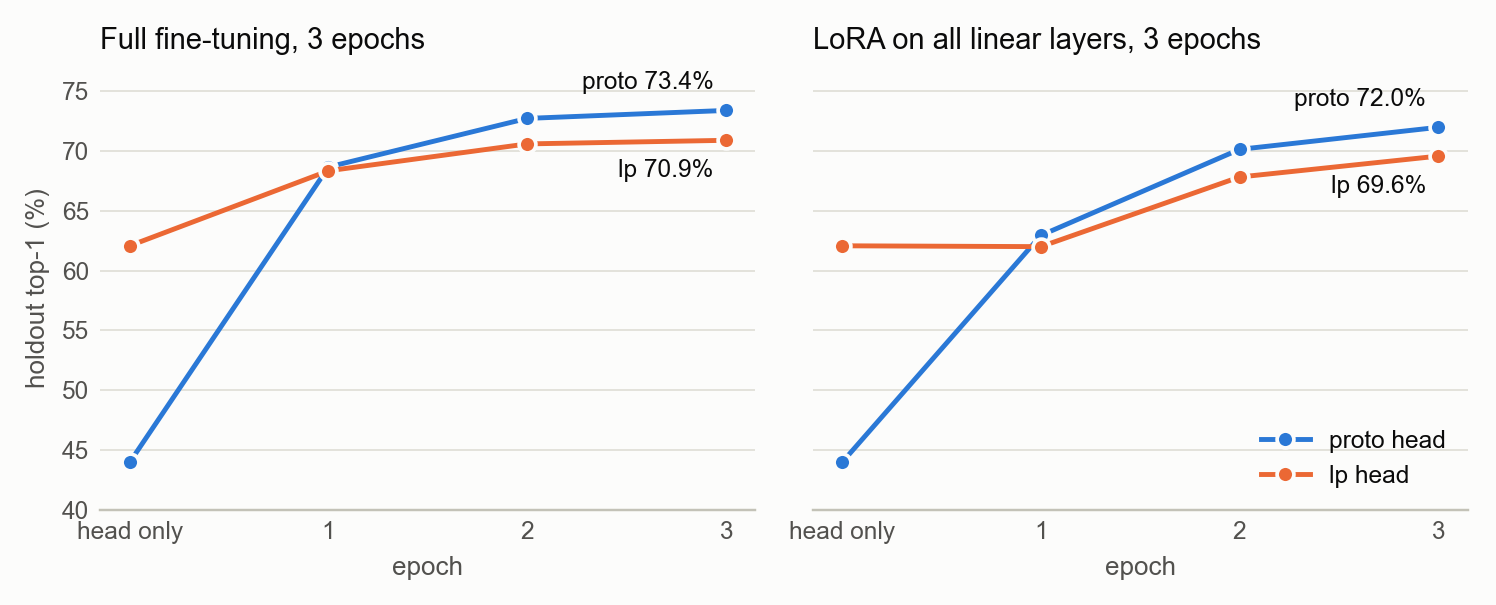
\includegraphics[width=0.8\linewidth]{figures/fig2_head_init_holdout.png}
  \caption{\textbf{Holdout accuracy during training for the LP and prototype heads} (3 epochs; left: full fine-tuning, right: LoRA on all linear layers).
  ``head only'' is the accuracy of the starting head before any training.
  The LP head starts 18 points higher but ends about 2.5 points lower.
  Points are the holdout checks after each epoch; for LoRA with the LP head, the final check after merging gives 69.45 (\cref{tab:head}) instead of 69.56.}
  \label{fig:head-curves}
\end{figure}

\begin{figure}[t]
  \centering
  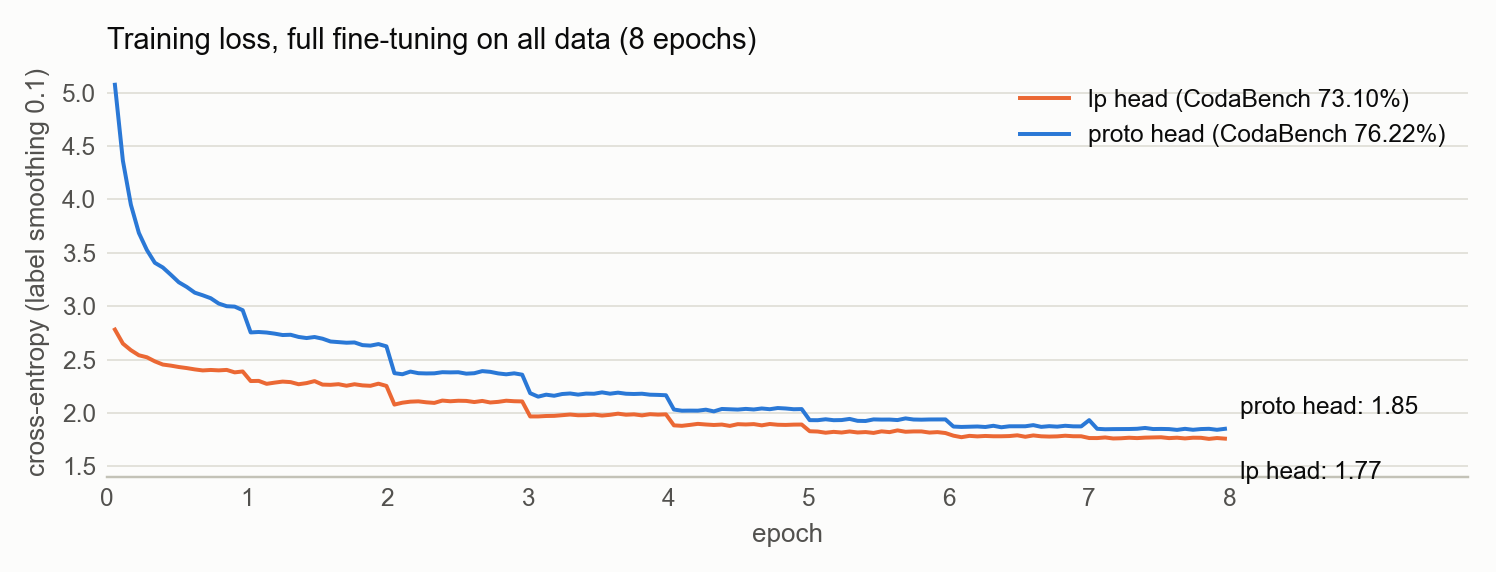
\includegraphics[width=0.8\linewidth]{figures/fig3_loss_lp_vs_proto.png}
  \caption{\textbf{Training loss of full fine-tuning on all data (8 epochs) with the LP and prototype heads}; nothing else differs.
  The prototype model has a \emph{higher} training loss (1.85 \vs 1.77 in the last epoch) but scores 3.12 points higher on the validation set.
  The loss drops at each epoch boundary and stays flat within an epoch, a sign that the model memorizes the 45 images per class.}
  \label{fig:loss}
\end{figure}

\Cref{tab:head} compares the three head starts in four settings.
In all four, the LP head is clearly the worst, 2.1--3.1 points below the prototype head, although it starts 18 points higher (\cref{fig:head-curves}).
For LoRA, the random and prototype heads end up level (71.95\% \vs 72.00\%), but the prototype head learns faster: it is 5 points ahead after the first epoch (63.3\% \vs 58.4\%).

\paragraph{Why does the LP head hurt?}
The probe was trained on \emph{the same images that are then used for fine-tuning}, so it already fits them well.
Over the first 100 steps of the LoRA runs, the mean training loss is 2.29 with the LP head, against 4.39 with the prototype head and 9.28 with a random head.
So the backbone gets only a small training signal, mostly from the few images the probe gets wrong.
When the features start to change, the trained head no longer matches them: in the LoRA run with the LP head, the training loss goes up from 2.22 to 2.69 during the first epoch, before any image is seen twice.
\Cref{fig:loss} shows the same for full fine-tuning: with the same settings, the LP model reaches a lower training loss but a much lower validation accuracy, so it memorizes more and generalizes less.
The random head is our control: it knows nothing about the classes, yet it does as well as the prototype head.
So the prototype head is not special; what hurts is a head that was trained on the training images.
LP-FT \citep{kumar2022lpft} uses the probe so that a random head does not distort the pretrained features, mainly to keep accuracy on new domains.
In our task the features have to change, and a random head did no harm.

\subsection{Comparing adaptation methods}
\label{sec:compare}

\begin{table}[t]
  \caption{\textbf{Seven adaptation methods under one protocol} (prototype head, 3 epochs, holdout top-1, \%). Params: trainable backbone share; img/s: training throughput; GB: peak training memory; ms: batch-1 latency.
  $^*$Peak during feature extraction; training used less.
  $^\dagger$Full fine-tuning recipe; $K = 1, 2$ use learning rate $3{\times}10^{-4}$ without layer decay or drop path.
}
  \label{tab:compare}
  \centering
  \footnotesize
  \setlength{\tabcolsep}{6pt}
  \begin{tabular}{@{}lrrrrr@{}}
    \toprule
    Method & Params & Holdout & img/s & GB & ms \\
    \midrule
    Linear probe & 0 & 61.94 & -- & 3.2 & 6.96 \\
    Partial, $K = 1$ & 8.26\% & 67.97 & 1,706 & 3.8$^*$ & 7.92 \\
    Partial, $K = 2$ & 16.5\% & 70.99 & 1,655 & 4.1 & 7.41 \\
    Partial, $K = 4^\dagger$ & 33.0\% & 71.88 & 1,611 & 7.0 & 7.41 \\
    Partial, $K = 6^\dagger$ & 49.6\% & 72.89 & 1,650 & 10.0 & 7.42 \\
    Full fine-tuning & 100\% & \textbf{73.38} & 1,139 & 18.9 & 7.78 \\
    \midrule
    BitFit & 0.120\% & 69.81 & 1,407 & 12.7 & 7.33 \\
    Adapter & 1.387\% & 71.54 & 1,509 & 12.8 & 9.74 \\
    AdaptFormer & 1.387\% & 71.17 & 1,436 & 12.8 & 10.23 \\
    LoRA, all linear & 1.375\% & \textbf{71.98} & 888 & 19.9 & 7.61 \\
    \bottomrule
  \end{tabular}
\end{table}

\begin{figure}[t]
  \centering
  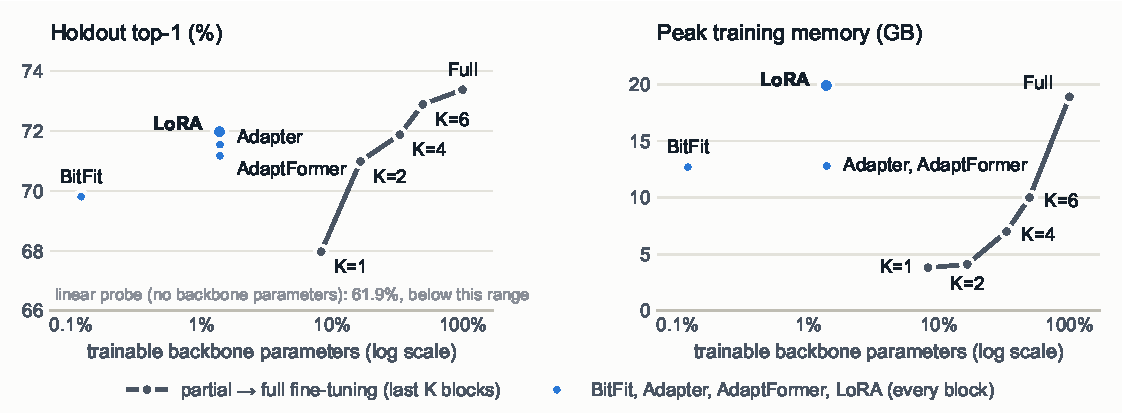
\includegraphics[width=\linewidth]{figures/fig4_methods_params.pdf}
  \caption{\textbf{Holdout accuracy (left) and peak training memory (right) against the share of trainable backbone parameters} (log scale) for the runs in \cref{tab:compare}.
  Methods that change every block (blue) get more accuracy per parameter than fine-tuning the last $K$ blocks (gray), but need more memory, because their gradients go back to the first block.
  The linear probe (61.9\%) is below the left panel; the memory of $K = 1$ is the feature-extraction peak.}
  \label{fig:params}
\end{figure}

To compare the methods fairly, we ran all seven with the same protocol: the prototype head, 3 epochs, the same holdout split and the same GPU (\cref{tab:compare,fig:params}).
All efficient methods use learning rate $10^{-3}$; we did not tune it for each method.

\paragraph{Where to train.}
Small changes in every block give much more accuracy per parameter than fine-tuning the top blocks.
BitFit trains 0.12\% of the backbone and beats fine-tuning the last block (8.3\%) by 1.8 points; LoRA (1.375\%) matches the last four blocks (33\%), and the Adapter (1.387\%) beats the last two (16.5\%).
Each extra top block helps less (the first adds 6.0 points over the linear probe, the second 3.0, each further pair about 1), likely because frozen lower blocks cannot change their features for the new classes, while small changes in every block reach all of them.
Among the efficient methods, LoRA is the most accurate (71.98\%), followed by the Adapter (71.54\%), AdaptFormer (71.17\%) and BitFit (69.81\%).
But LoRA is only 0.44 points ahead of the Adapter, close to our noise level; its clear advantage is that it can be merged.
The serial Adapter and the parallel AdaptFormer differ by 0.37 points, and they also use different scales (1.0 \vs 0.1), so we cannot say which placement is better.
None reaches full fine-tuning (73.38\%), although the project description expects parameter-efficient methods to do better on small data; one possible reason is that each class has few images, but the whole training set has 450,000, enough to fine-tune the full backbone.

\paragraph{Training memory.}
Training memory depends on how far back the gradients have to go, not on how many parameters are trained (\cref{fig:params}, right).
Partial fine-tuning adds about 1.5\,GB per trained block, which extrapolates to 18.8\,GB for all 12 blocks, the same as full fine-tuning (18.9\,GB).
BitFit and the two adapters train at most 1.4\% of the backbone but need 12.7--12.8\,GB, more than fine-tuning half the network ($K = 6$, 10.0\,GB), because their gradients must reach the first block.
They still use a third less memory than full fine-tuning and train 24--32\% faster, since frozen weight matrices need no weight gradients; LoRA is the exception (\cref{sec:ablation-lora}).
At inference, only the two adapters cost extra: 9.74 and 10.23\,ms at batch size 1, against 7.33\,ms for the plain model.

\subsection{LoRA: where to add capacity, and how long to train}
\label{sec:ablation-lora}

\Cref{tab:peft,tab:length} in the appendix give the numbers.
\textbf{Capacity mattered more than the learning rate.}
With the LP head, halving the LoRA learning rate changed nothing (\minus0.12), while adding LoRA to all four linear layers instead of only \texttt{qkv} added 0.88 points.
\textbf{LoRA is not cheaper to train here.}
LoRA on all linear layers trains slower than full fine-tuning (885 \vs 1,131 img/s) and needs slightly more memory (19.9 \vs 18.9\,GB).
To train its $A$ matrices, it must store the input of every linear layer, as full fine-tuning does, plus the activations of its 96 extra small matrix products; its savings are in stored size (35.5\,MB \vs 374\,MB per checkpoint).
\textbf{Longer training helps full fine-tuning but not LoRA.}
Going from 3 to 8 epochs adds 2.21 points for the final full fine-tuning recipe.
LoRA stops improving after about 3 epochs, and with the prototype head 6 epochs are worse than 3 (\minus0.46), although its training loss keeps falling (1.95 to 1.70).
We think the head is the cause: it holds 7.69M of LoRA's 8.87M trainable parameters, and compared with full fine-tuning our LoRA recipe trains it with a 10$\times$ higher learning rate, a 500$\times$ smaller weight decay and no drop path, so with more epochs it mostly memorizes the 43 images per class (not yet tested).

\subsection{After the deadline: input resolution}
\label{sec:post}

\begin{table}[t]
  \caption{\textbf{Input resolution} (after the deadline; full fine-tuning, prototype head, 3 epochs, holdout top-1, \%; runs \run{1019\_1120\_1\_full} and \run{1105\_1031\_1\_full\_288}). Position embeddings are interpolated to the patch grid of each size. Bold: best test size for each model.}
  \label{tab:res}
  \centering
  \footnotesize
  \setlength{\tabcolsep}{6pt}
  \begin{tabular}{@{}lrrrrrrrr@{}}
    \toprule
    & \multicolumn{6}{c}{Test size (pixels)} & & \\
    \cmidrule(lr){2-7}
    Trained at & 224 & 256 & 288 & 320 & 352 & 384 & GPU-h & GB \\
    \midrule
    224 pixels & 73.38 & 75.21 & \textbf{75.50} & 75.28 & 74.33 & 72.94 & 0.48 & 18.9 \\
    288 pixels & 73.10 & 75.74 & 77.23 & \textbf{77.78} & 77.63 & 77.41 & 0.68 & 30.2 \\
    \bottomrule
  \end{tabular}
\end{table}

After the deadline, the gap to the top teams on the leaderboard made us ask what still limits our models, so we changed only the image size, with the backbone and protocol of \cref{tab:compare}.
timm interpolates the $14{\times}14$ position embeddings to the patch grid of the input ($18{\times}18$ at 288 pixels), so no parameter is added (\cref{tab:res}).
Testing our 224-pixel model at 288 pixels adds 2.1 points with no retraining.
FixRes \citep{touvron2019fixres} explains this: random-resized crops make objects look larger during training, so slightly larger test images match them better.
Training at 288 pixels adds another 2.3 points, and the best test size moves up to 320 pixels: 77.78\%, 4.4 points above the 224-pixel model.
This 3-epoch run still fits the budget (0.68 GPU-hours), but needs 30.2\,GB instead of 18.9\,GB, because a 288-pixel image has 325 tokens instead of 197.
We also trained the full 8-epoch recipe at 288 pixels on all images; it takes 1.61 GPU-hours, over the budget, and has no test score, so it is not one of our results.
Input resolution gave the largest gain we found, but we found it too late.

\section{Conclusion}
\label{sec:conclusion}

When adapting ViT-B/16 to 10,000 classes with 45 images each, the biggest gain came from how we started the new head, not from the adaptation method: class prototypes instead of a linear probe added 2.1--3.1 points, and gave 76.09\% (full fine-tuning) and 71.67\% (LoRA, 1.375\% of the backbone) on the test set.
Across seven methods, small changes in every block gave more accuracy per parameter than fine-tuning whole top blocks, with 12--69$\times$ fewer parameters, and training memory followed how far back the gradients go.

\paragraph{What we learned.}
First, failed ideas helped: halving LoRA's learning rate changed nothing, which pointed us from the optimizer to the head, and training LoRA longer lowered its training loss but also its accuracy, which showed that memorization, not underfitting, limits it.
Second, a good start can be misleading: the linear-probe head starts 18 points ahead and ends 2.5 points behind, so we judged every choice on held-out data after training, never on the training loss or the starting accuracy.
Third, we studied the adaptation method early and the input late: after the deadline, larger input images added 4.4 holdout points (\cref{sec:post}), more than any single adaptation choice.

\paragraph{Limitations and next steps.}
Each setting was trained once (seed 0), and the holdout noise is about $\pm$0.3 points, so small differences, such as the 0.26-point gain from two extra images per class, are uncertain.
Our explanation of why the linear-probe head hurts fits the loss curves and the random-head control, but it is not a full proof.
The efficient methods share one learning rate that we did not tune per method, we only used LoRA rank 8, and some pairs (partial $K = 1, 2$ \vs $4, 6$; Adapter \vs AdaptFormer) differ in more than one setting.
Next, we would trade epochs for image size within the budget (\eg 6 epochs at 224 pixels and 2 at 288, about 1.2 GPU-hours by our estimate), test a lower head learning rate for LoRA, and try prompt-based methods.


\bibliography{refs}
\bibliographystyle{iclr2026_conference}

% Appendix: training-log excerpts, all runs, extra tables and hyperparameters (after the references)
\clearpage
\raggedbottom % no stretched gaps on appendix pages with tables
\appendix

\section{Training-log excerpts}
\label{sec:logs}

The project asks us to back up training time and VRAM with training logs.
Below are parts of \texttt{train\_log.txt} for our two final models; the full logs (every 100 steps) are available on request.
Dates are removed from the timestamps, Google Drive paths are shortened, and long lines are wrapped.
GPU-hours include head initialization (feature extraction), training and the holdout check after every epoch (\cref{sec:budget}).

\paragraph{Final full fine-tuning model} (prototype head, all 45 images per class, 8 epochs, flip TTA at prediction):
{\scriptsize
\begin{verbatim}
========== 1019_1319_1_full ==========
[13:32:14] full: lr 0.0001, head lr 0.0001, wd 0.05, layer decay 0.75, epochs 8,
           holdout 0/class, head init proto, time budget 1.20 h
[13:32:14] Environment: NVIDIA A100-SXM4-80GB (80 GB), bfloat16, 12 CPUs |
           torch 2.11.0+cu130 (CUDA 13.0), timm 1.0.30, peft 0.21.1
[13:38:32] Extracted features for 450,000 train / 0 holdout images in 6.1 min
[13:38:32] Head initialized from proto (6.2 min incl. feature extraction,
           counted in this run's GPU time)
[13:38:32] Trainable (excl. head): 85,798,656 = 100.000% of backbone |
           head 7,690,000 params (fine-tuned)
[13:38:32] Training up to 8 epochs x 1757 steps (batch 256x1, warmup 1757 steps)
[13:40:03] Speed 1146 img/s, 6.5 min/epoch
[13:46:13] == epoch 1: train loss 3.4158, 13.8 min used
[13:52:55] == epoch 2: train loss 2.6899, 20.5 min used
[13:59:51] == epoch 3: train loss 2.3729, 27.4 min used
[14:06:42] == epoch 4: train loss 2.1758, 34.2 min used
[14:13:40] == epoch 5: train loss 2.0321, 41.1 min used
[14:20:31] == epoch 6: train loss 1.9367, 47.9 min used
[14:27:32] == epoch 7: train loss 1.8741, 54.9 min used
[14:34:26] == epoch 8: train loss 1.8491, 61.8 min used
[14:34:29] Training done: 14056 steps, 1.03 GPU-hours (budget 1.20 h)
[14:34:29] Peak VRAM: 18.9 GB allocated, 20.1 GB reserved by PyTorch (GPU has 80 GB)
[14:34:32] Inference latency (batch 1): 14.95 ms/img | throughput (batch 256): 1919 img/s |
           NVIDIA A100-SXM4-80GB, bfloat16, with flip TTA
[14:35:29] [val] 50,000 predictions over 9,992 classes (max 13 per class) ->
           .../submission_val_1019_1319_1_full.zip
\end{verbatim}
}

\paragraph{Final LoRA model} (LoRA on all linear layers, prototype head, 3 epochs, 2 images per class held out, no TTA):
{\scriptsize
\begin{verbatim}
========== 1019_1319_3_lora ==========
[14:57:51] lora: lr 0.001, head lr 0.001, wd 0.0001, layer decay 1.0, epochs 3,
           holdout 2/class, head init proto, time budget 1.20 h
[14:57:51] Environment: NVIDIA A100-SXM4-80GB (80 GB), bfloat16, 12 CPUs |
           torch 2.11.0+cu130 (CUDA 13.0), timm 1.0.30, peft 0.21.1
[15:06:07] Extracted features for 430,000 train / 20,000 holdout images in 7.2 min
[15:06:08] Prototype head (zero-shot, 0 trainable params): holdout top-1 44.01%
[15:06:08] Head initialized from proto (7.2 min incl. feature extraction,
           counted in this run's GPU time)
[15:07:15] Trainable (excl. head): 1,179,648 = 1.375% of backbone |
           head 7,690,000 params (fine-tuned)
[15:07:15] Training up to 3 epochs x 1679 steps (batch 256x1, warmup 503 steps)
[15:07:53] Speed 888 img/s, 8.1 min/epoch
[15:15:44] == epoch 1: train loss 3.2174, holdout top-1 62.94%, 15.7 min used
[15:24:12] == epoch 2: train loss 2.4125, holdout top-1 70.12%, 24.2 min used
[15:32:40] == epoch 3: train loss 1.9496, holdout top-1 71.97%, 32.6 min used
[15:32:41] Training done: 5037 steps, 0.54 GPU-hours (budget 1.20 h)
[15:32:41] Peak VRAM: 19.9 GB allocated, 21.3 GB reserved by PyTorch (GPU has 80 GB)
[15:33:00] Final holdout: top-1 71.98%, top-5 89.07%
[15:33:03] Inference latency (batch 1): 7.61 ms/img | throughput (batch 256): 3869 img/s |
           NVIDIA A100-SXM4-80GB, bfloat16, no flip TTA
[15:33:55] [val] 50,000 predictions over 9,991 classes (max 15 per class) ->
           .../submission_val_1019_1319_3_lora.zip
\end{verbatim}
}

\section{All runs}
\label{sec:all-runs}

\begin{table}[H]
  \caption{\textbf{All 26 runs.} IDs encode the batch start time (month, day, hour, minute) and the position in the batch; the last block is the method comparison (\cref{sec:compare}).
  LoRA all: LoRA on all linear layers. Trainable: backbone parameters without the 7.69M head. GB: peak allocated training memory ($K = 1$: feature extraction). ms: batch-1 latency.
  $^\ddagger$Flip TTA. $^*$RTX PRO 6000 Blackwell; all other runs on an A100-SXM4-80GB (speed and latency are not comparable).
  The LP head (62.07\%) is computed inside every LP run; \run{1102\_1149\_2} re-ran it alone.}
  \label{tab:all-runs}
  \centering
  \scriptsize
  \setlength{\tabcolsep}{2.5pt}
  \resizebox{\linewidth}{!}{%
  \begin{tabular}{@{}lllrrrrrrr@{}}
    \toprule
    Run & Method & Head & Ep. & Trainable & Holdout & Val & GPU-h & GB & ms \\
    \midrule
    \run{0928\_0636\_1\_linear} & Zero-shot & prototype & 0 & 0 & 43.95 & -- & 0.11 & 3.9 & 7.55 \\
    \run{0928\_0636\_3\_full} & Full FT & LP & 3 & 100\% & 70.88 & -- & 0.45 & 18.9 & 7.31 \\
    \run{0928\_0748\_1\_full} & Full FT & LP & 8 & 100\% & 72.31 & 72.57/72.84$^\ddagger$ & 1.03 & 18.9 & 7.35 \\
    \run{1018\_2306\_1\_full} & Full FT, all data & LP & 8 & 100\% & -- & 73.10$^\ddagger$ & 1.03 & 18.9 & 14.92$^\ddagger$ \\
    \run{1019\_1120\_1\_full} & Full FT & prototype & 3 & 100\% & 73.38 & -- & 0.48 & 18.9 & 7.78 \\
    \run{1019\_1319\_2\_full} & Full FT, all data & prototype & 3 & 100\% & -- & 74.01$^\ddagger$ & 0.44 & 18.9 & 15.24$^\ddagger$ \\
    \run{1019\_1319\_1\_full} & \textbf{Full FT, all data (final)} & prototype & 8 & 100\% & -- & \textbf{76.22}$^\ddagger$ & 1.03 & 18.9 & 14.95$^\ddagger$ \\
    \midrule
    \run{0928\_0636\_2\_lora} & LoRA qkv & LP & 3 & 0.344\% & 68.57 & -- & 0.40 & 13.5 & 7.22 \\
    \run{0928\_0748\_2\_lora} & LoRA qkv, head lr $2{\times}10^{-4}$ & LP & 10 & 0.344\% & 68.69 & -- & 1.06 & 13.5 & 7.53 \\
    \run{1018\_1239\_1\_lora} & LoRA qkv, lr $5{\times}10^{-4}$ & LP & 3 & 0.344\% & 68.45 & -- & 0.41 & 13.5 & 7.15 \\
    \run{1018\_1239\_3\_adaptformer} & AdaptFormer & LP & 3 & 1.387\% & 69.05 & -- & 0.39 & 12.8 & 9.89 \\
    \run{1018\_1239\_2\_lora} & LoRA all & LP & 3 & 1.375\% & 69.45 & -- & 0.55 & 19.9 & 7.03 \\
    \run{1018\_2306\_2\_lora} & LoRA all & LP & 6 & 1.375\% & 69.87 & -- & 0.97 & 19.9 & 7.31 \\
    \run{1019\_0953\_1\_lora}$^*$ & LoRA all & random & 3 & 1.375\% & 71.95 & -- & 0.37$^*$ & 19.9 & 1.81$^*$ \\
    \run{1019\_0953\_2\_lora}$^*$ & LoRA all & prototype & 3 & 1.375\% & 72.00 & -- & 0.44$^*$ & 19.9 & 1.82$^*$ \\
    \run{1019\_1120\_2\_lora} & LoRA all & prototype & 6 & 1.375\% & 71.52 & -- & 0.97 & 19.9 & 7.76 \\
    \run{1019\_1319\_3\_lora} & \textbf{LoRA all (final)} & prototype & 3 & 1.375\% & \textbf{71.98} & \textbf{71.90} & 0.54 & 19.9 & 7.61 \\
    \midrule
    \run{1102\_1149\_1\_linear\_proto} & Zero-shot (re-run) & prototype & 0 & 0 & 43.95 & -- & 0.10 & 3.8 & 7.32 \\
    \run{1102\_1149\_2\_linear\_lp} & Linear probe & LP & -- & 0 & 61.94 & -- & 0.10 & 3.2 & 6.96 \\
    \run{1102\_1942\_1\_partial\_k1} & Partial FT, $K = 1$ & prototype & 3 & 8.263\% & 67.97 & -- & 0.35 & 3.8 & 7.92 \\
    \run{1102\_1942\_2\_partial\_k2} & Partial FT, $K = 2$ & prototype & 3 & 16.524\% & 70.99 & -- & 0.35 & 4.1 & 7.41 \\
    \run{1102\_1942\_3\_partial\_k4} & Partial FT, $K = 4$ & prototype & 3 & 33.046\% & 71.88 & -- & 0.35 & 7.0 & 7.41 \\
    \run{1102\_1942\_4\_partial\_k6} & Partial FT, $K = 6$ & prototype & 3 & 49.568\% & 72.89 & -- & 0.35 & 10.0 & 7.42 \\
    \run{1102\_2023\_1\_bitfit} & BitFit & prototype & 3 & 0.120\% & 69.81 & -- & 0.39 & 12.7 & 7.33 \\
    \run{1102\_2017\_1\_adapter} & Adapter & prototype & 3 & 1.387\% & 71.54 & -- & 0.37 & 12.8 & 9.74 \\
    \run{1102\_2212\_1\_adaptformer} & AdaptFormer & prototype & 3 & 1.387\% & 71.17 & -- & 0.39 & 12.8 & 10.23 \\
    \bottomrule
  \end{tabular}}
\end{table}

\paragraph{Runs after the deadline (\cref{sec:post}).}
None of them is used for a ranked result.
Batch \run{1105\_0141} ran zero-shot and the linear probe with the ImageNet-21k-only checkpoints \nolinkurl{augreg_in21k} and \nolinkurl{orig_in21k} (zero-shot 49.96\% and 42.43\%, linear probe 61.05\% and 51.07\%; \cref{sec:budget}), and evaluated \run{1019\_1120\_1\_full} at six test sizes.
\run{1105\_1031\_1\_full\_288} trains 3 epochs at 288 pixels on the holdout split (0.68 GPU-h, 30.2\,GB).
\run{1105\_1032\_1\_full\_288} trains the final recipe at 288 pixels on all images (1.61 GPU-h, 30.2\,GB); it was not submitted, so it has no test score.

\section{Hardware, software and the path to the final model}
\label{sec:hardware}

All runs use one NVIDIA A100-SXM4-80GB with 12 CPU cores, except one ablation batch (random and prototype heads for LoRA in \cref{tab:head}), which ran on an RTX PRO 6000 Blackwell.
Repeating its prototype run on the A100 gave 71.98\% \vs 72.00\%, so accuracies are comparable across the two GPUs; speeds and latencies are not.
Software, as logged from batch \run{1019\_1120} on, which covers all final models and the method comparison: PyTorch 2.11.0 (CUDA 13.0), timm 1.0.30 and PEFT 0.21.1. Earlier runs used the then-current releases, which were not logged.
Peak memory is the memory allocated by PyTorch; the memory it reserved is 0.2--1.4\,GB higher (20.1\,GB for the final model).
\Cref{fig:progression} shows the validation accuracy of the final full fine-tuning recipe as we changed one setting at a time.

\begin{figure}[H]
  \centering
  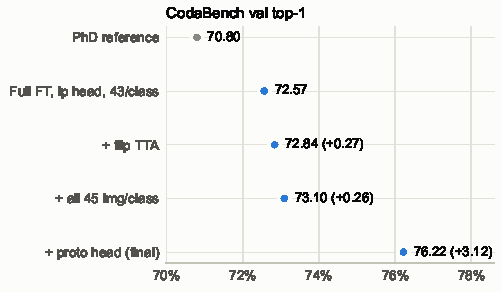
\includegraphics[width=0.6\linewidth]{figures/fig1_codabench_progression_col.pdf}
  \caption{\textbf{CodaBench validation accuracy as we change one setting at a time} (all runs: full fine-tuning, 8 epochs). The gray dot is the reference. Positions encode values, so the axis starts at 70\%.}
  \label{fig:progression}
\end{figure}

\section{Extra tables}
\label{sec:ablation-tables}

\Cref{tab:params} shows how the trainable parameters of each method are counted (\cref{sec:peft}).
\Cref{tab:peft,tab:length} give the numbers behind \cref{sec:ablation-lora}.

\begin{table}[H]
  \caption{\textbf{Trainable backbone parameters} (head excluded; $r = 8$; partial: $K \in \{1, 2, 4, 6\}$).
  1,536: final LayerNorm (partial) or the patch-embedding and final-norm biases (BitFit); 8,448 biases per block.
  Adapter: $2 \cdot 768 \cdot 64 + 64 + 768 = 99{,}136$ per block.
  LoRA adds $r\,(d_\text{in} + d_\text{out})$ per layer, \ie $3{,}072\,r$ for qkv and $12{,}288\,r$ for qkv, proj, fc1 and fc2 together.}
  \label{tab:params}
  \centering
  \footnotesize
  \begin{tabular}{@{}llrr@{}}
    \toprule
    Method & Count & Parameters & \% \\
    \midrule
    Partial, last $K$ blocks & $7{,}087{,}872\,K + 1{,}536$ & 7.09M--42.5M & 8.26--49.6 \\
    Full fine-tuning & all & 85,798,656 & 100 \\
    BitFit & $12 \cdot 8{,}448 + 1{,}536$ & 102,912 & 0.120 \\
    Adapter, AdaptFormer & $12 \cdot 99{,}136$ & 1,189,632 & 1.387 \\
    LoRA, qkv only & $12 \cdot 3{,}072\,r$ & 294,912 & 0.344 \\
    LoRA, all linear & $12 \cdot 12{,}288\,r$ & 1,179,648 & 1.375 \\
    \bottomrule
  \end{tabular}
\end{table}

\begin{table}[H]
  \caption{\textbf{PEFT design} (LP head, 3 epochs, holdout top-1, \%). Params: trainable backbone parameters (head excluded). img/s: training throughput; GB: peak training memory; ms: batch-1 latency after merging (A100, bf16).}
  \label{tab:peft}
  \centering
  \footnotesize
  \setlength{\tabcolsep}{5pt}
  \begin{tabular}{@{}lrrrrr@{}}
    \toprule
    Method & Params & Holdout & img/s & GB & ms \\
    \midrule
    LoRA qkv, lr $10^{-3}$ & 0.344\% & 68.57 & 1,341 & 13.5 & 7.22 \\
    LoRA qkv, lr $5{\times}10^{-4}$ & 0.344\% & 68.45 & 1,353 & 13.5 & 7.15 \\
    LoRA all linear & 1.375\% & \textbf{69.45} & 885 & 19.9 & 7.03 \\
    AdaptFormer & 1.387\% & 69.05 & 1,437 & 12.8 & 9.89 \\
    \midrule
    Full fine-tuning & 100\% & 70.88 & 1,131 & 18.9 & 7.31 \\
    \bottomrule
  \end{tabular}
\end{table}

\begin{table}[H]
  \caption{\textbf{Training length} (holdout top-1, \%; LoRA all: LoRA on all linear layers).
  $^\ddagger$All 45 images per class with flip TTA, CodaBench validation.
  $^\dagger$The 10-epoch run also lowered the head learning rate to $2{\times}10^{-4}$.}
  \label{tab:length}
  \centering
  \footnotesize
  \setlength{\tabcolsep}{5pt}
  \begin{tabular}{@{}lrrr@{}}
    \toprule
    Setting & Short (ep) & Long (ep) & $\Delta$ \\
    \midrule
    Full FT, LP & 70.88 (3) & 72.31 (8) & $+$1.43 \\
    Full FT, prototype, final$^\ddagger$ & 74.01 (3) & 76.22 (8) & $+$2.21 \\
    LoRA qkv, LP$^\dagger$ & 68.57 (3) & 68.69 (10) & $+$0.12 \\
    LoRA all, LP & 69.45 (3) & 69.87 (6) & $+$0.42 \\
    LoRA all, prototype & 71.98 (3) & 71.52 (6) & \minus0.46 \\
    \bottomrule
  \end{tabular}
\end{table}

\section{Hyperparameters}
\label{sec:hparams}

\begin{table}[H]
  \caption{\textbf{Hyperparameters.} Weight decay is not applied to biases, normalization parameters, the class token and position embeddings. Evaluation resizes to 248 pixels and takes a 224 center crop.}
  \label{tab:hparams}
  \centering
  \scriptsize
  \renewcommand{\arraystretch}{1.05}
  \setlength{\tabcolsep}{3pt}
  \begin{tabular}{@{}>{\raggedright}p{1.8cm}>{\raggedright}p{2.9cm}>{\raggedright}p{3.0cm}>{\raggedright}p{2.6cm}>{\raggedright\arraybackslash}p{2.4cm}@{}}
    \toprule
    & Full fine-tuning & LoRA & AdaptFormer & Linear-probe head \\
    \midrule
    Trainable & all weights + head & $A, B$ in qkv, proj, fc1, fc2 (all 12 blocks) + head & parallel MLP adapters + head & head only, on cached features \\
    Method-specific & layer-wise lr decay 0.75, drop path 0.1 & $r=8$, $\alpha=16$, no dropout, no layer decay, no drop path, merged after training & bottleneck 64, scale 0.1, dropout 0.1 & starts from the prototype head \\
    Optimizer & AdamW & AdamW & AdamW & AdamW \\
    Learning rate & $10^{-4}$ (head $10^{-4}$) & $10^{-3}$ (head $10^{-3}$) & $10^{-3}$ (head $10^{-3}$) & $10^{-3}$ \\
    Weight decay & 0.05 & $10^{-4}$ & $10^{-4}$ & $10^{-4}$ \\
    Schedule & \multicolumn{3}{p{8.9cm}}{linear warmup (1 epoch; 0.3 epochs for 3-epoch runs), then cosine decay to 0} & cosine, no warmup \\
    Epochs & 3 or 8 & 3, 6 or 10 & 3 & 10 \\
    Batch size & 256 & 256 & 256 & 4,096 \\
    Precision & bf16 & bf16 & bf16 & fp32 head, fp16 features \\
    Regularization & \multicolumn{3}{p{8.9cm}}{label smoothing 0.1, gradient clipping at norm 1.0} & label smoothing 0.1 \\
    Augmentation & \multicolumn{3}{p{8.9cm}}{RandomResizedCrop (scale 0.25--1) + horizontal flip} & none (center crops) \\
    \bottomrule
  \end{tabular}
\end{table}

Methods added for \cref{sec:compare} train for 3 epochs with the settings above, except: partial fine-tuning uses learning rate $3{\times}10^{-4}$ and weight decay 0.05 for $K = 1, 2$ and the full fine-tuning settings for $K = 4, 6$ (drop path only in trained blocks); BitFit uses learning rate $10^{-3}$ and no weight decay; the Adapter is AdaptFormer's bottleneck placed after the MLP, with scale 1.0.


\end{document}
